\documentclass{article}
\usepackage{graphicx}
\topmargin=0.0in %length of margin at the top of the page (1 inch added by default)
\oddsidemargin=0.0in %length of margin on sides for odd pages
\evensidemargin=0in %length of margin on sides for even pages
\textwidth=6.5in %How wide you want your text to be
\marginparwidth=0.5in
\headheight=0pt %1in margins at top and bottom (1 inch is added to this value by default)
\headsep=0pt %Increase to increase white space in between headers and the top of the page
\textheight=9.0in %How tall the text body is allowed to be on each page
\newcommand\tab[1][3cm]{\hspace*{#1}}
 \begin{document}

 \begin{center}
 	 {
 	 	\large { KEYUR H. RAKHOLIYA}
 	 }
 	
 \end{center}
   \hline
 \begin{flushleft}
 	19,Rohini society, 		\hspace{2.8in}    		    Contact: 75679 25394            \\
 	Vaniyawad circle, 		\hspace{2.8in}		    	e-mailid: keyurrakholiya302@gmail.com
 	College Road, \\
	Nadiad-387001,     \\
 	Gujarat       \\
 \end{flushleft}
 \vspace{-0.3in}

 \begin{figure}[h]
    \hspace{4.4in}
	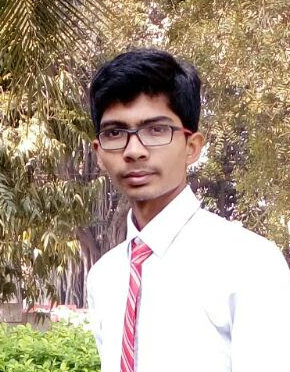
\includegraphics[width=90px]{keyur}
 \end{figure}
 
 %%%%%%%%%%%%%  OBJECTIVE   %%%%%%%%%%%
 \begin{flushleft}
 	\textbf{OBJECTIVE}
 	
 	\vspace{-0.20in}
 	\hspace{1.5in}
 	having experience in embedded system since TWO year. looking forward to develop a system which can reduce human efforts.
 \end{flushleft}
 
 %%%%%%%%%%%%   EDUCATION   %%%%%%%%%
 \begin{flushleft}
 	\textbf{EDUCATION}
 	\hspace{0.45in}
 	\begin{tabular}{|c|c|c|c|c|}
 		\hline
 		Degree & School & University & Passing year & Pass   \\
 		&        &            &              & Percentage\\
 		\hline
 		
 		B.tech & Noble high school, & Dharmsingh Desai & 2018 &8.01 SPI\\
 	E.C.E	&Junagadh & University,Nadiad& & \\
 		\hline
 	\end{tabular}
 \end{flushleft}
 
 %%%%%%%%%%%%%%%   PROJECTS     %%%%%%%%%%5
 \begin{flushleft} 
 	\vspace{0.2in}
 	\textbf{PROJECTS}
 	\begin{enumerate}
 		\vspace{-0.29in}
 		\addtolength{\itemindent}{1.359in}
 		\item  Autonomous Robot on PIZZA Delivery Theme in e-YANTRA'15
 		\item  Line follower robot without micro controller.
 		\item  Arduino uno base projects.
 	\end{enumerate}
 \end{flushleft}
 
 %%%%%%%%%%%%  		training and internship 	%%%%%%%%
 \begin{flushleft} 
 	\vspace{0.4in}
 	\textbf{TRAINING \& \\ INTERNSHIP}
 	\begin{itemize}
 		\vspace{-0.44in}
 		\addtolength{\itemindent}{1.359in}
 		\item  e-YANTRA Summer Internship -2016
 	\end{itemize}
 \end{flushleft}
 
  %%%%%%%%%%%%%%%%%%%%%%   Research and pub. %%%%%%%%%%
  \begin{flushleft} 
  	\vspace{0.4in}
  	\textbf{RESEARCH \\ PUBLICATION}
  	\begin{enumerate}
  		\vspace{-0.45in}
  		\addtolength{\itemindent}{1.359in}
  		\item  presented a chart on LOW COST OPTICAL FIBER COMMUNICATION KIT
  	\end{enumerate}
  \end{flushleft}
  
  %%%%%%%%%%%      technical skill %%%%%%%%	
   \begin{flushleft}
  \vspace{0.4in}
  \textbf{TECHNICAL  \\ SKILL}
  \begin{itemize}
  	\vspace{-0.45in}
  	\addtolength{\itemindent}{1.359in}
  	\item  Deep knowledge of circuit designing
  	\item  designing and implementation of electronics project
  	\item  programming language
  	{\begin{itemize}
  			\addtolength{\itemindent}{1.359in}
  			\item C language
  			\item embedded C
  			\item assembly language
  			\item C++
  			
  		\end{itemize}
  	}  
  	\item knowledge of micro controller
  	{\begin{itemize}
  			\addtolength{\itemindent}{1.359in}
  			\item 8051 
  			\item Arduino uno , Arduino mega
  			\item atmel ATMEGA2560
  			
  		\end{itemize}
  	}  
  	
  \end{itemize}
  \end{flushleft}

  	 	
  	 	%%%%%%%%%%		soft skill		%%%%%%%%
 \begin{flushleft} 
  	 		
  	 		\vspace{0.4in}
  	 		\textbf{SOFT SKILL}
  	 		\begin{enumerate}
  	 			\vspace{-0.30in}
  	 			\addtolength{\itemindent}{1.359in}
  	 			\item Communication skill
  	 			\item Leadership 
  	 			\item Management 
  	 			\item entrepreneurship
  	 		\end{enumerate}
  	 	\end{flushleft}
 
 	%%%%%%% 	extra curricular activities		%%%%%%%
 	\begin{flushleft} 
 		
 		
 		
 		\vspace{0.4in}
 		\textbf{EXTRA - \\CURRICULAR \\ACTIVITIES }
 		\begin{itemize}
 			\vspace{-0.65in}
 			\addtolength{\itemindent}{1.359in}
 			\item  managing people and Events
 			\item  arranging social activity seminars
 			
 		\end{itemize}
 	\end{flushleft}

 %%%%%%%		co curricullar activity	%%%%%%%
 \begin{flushleft} 
 	\vspace{0.4in}
 	\textbf{CO- \\CURRICULAR \\ACTIVITIES }
 	\begin{enumerate}
 		\vspace{-0.65in}
 		\addtolength{\itemindent}{1.359in}
 		\item  making videos for youtube channel 
 		\item  Playing Cricket
 		
 	\end{enumerate}
 \end{flushleft}

%%%%%%%%%%	personal details 	%%%%%%%

\begin{flushleft}
	\vspace{0.4in}
	\textbf{Personal Details} \hspace{0.36in}Father's name: \hspace{0.13in} HARASUKHBHAI D. RAKHOLIYA \\
	\hspace{1.55in}Mother's name: \hspace{0.08in} JAYABEN H. RAKHOLIYA\\
	\hspace{1.55in}Sex:\hspace{0.85in} MALE\\
	\hspace{1.55in}Date of birth:\hspace{0.255in} MARCH,16 1997	\\
	\hspace{1.55in}Nationality:\hspace{0.45in}INDIAN\\
	\hspace{1.55in}Marital status:\hspace{0.28in}SINGLE
	
\end{flushleft}

\end{document}